\documentclass[svgnames,11pt]{beamer}
\input{/home/tof/Documents/Cozy/latex-include/preambule_commun.tex}
\input{/home/tof/Documents/Cozy/latex-include/preambule_beamer.tex}
%\usepackage{pgfpages} \setbeameroption{show notes on second screen=left}
\author[]{Christophe Viroulaud}
\title{Programmation dynamique\\Rendu de monnaie}
\date{\framebox{\textbf{Algo 25}}}
%\logo{}
\institute{Terminale - NSI}

\begin{document}
\begin{frame}
\titlepage
\end{frame}

\begin{frame}
    \frametitle{}
    Pour répondre à un problème on peut utiliser plusieurs stratégies algorithmiques selon l'objectif à atteindre:
    \begin{itemize}
        \item trouver une solution exacte même si cela prend un temps long,
        \item trouver une solution approchée mais plus rapidement.
    \end{itemize}


\end{frame}
\begin{frame}
    \frametitle{}

    \begin{framed}
        \centering Peut-on trouver une solution optimale en un temps raisonnable?
    \end{framed}

\end{frame}
\section{Le rendu de monnaie}
\begin{frame}
    \frametitle{Le rendu de monnaie}

    \begin{aretenir}[Définition]
        Le problème du rendu de monnaie consiste à minimiser le nombre de pièces à rendre pour une somme donnée.\\On dispose d'un système de monnaie (exemple: système européen).
    \end{aretenir}

\end{frame}
\section{Approche gloutonne}
\subsection{Principe}
\begin{frame}
    \frametitle{Approche gloutonne - Principe}

    \begin{aretenir}[]
    La stratégie gloutonne est une méthode approchée de résolution. Elle consiste à faire un choix de résolution et ne pas revenir dessus.\\
    Dans le problème du rendu de monnaie, le choix est fait de rendre d'abord \textbf{la plus grande pièce possible}.
    \end{aretenir}

\end{frame}
\subsection{Algorithme}
\begin{frame}[fragile]
    \begin{activite}
Le système monétaire est donné dans l'ordre décroissant:
\begin{lstlisting}[language=Python , basicstyle=\ttfamily\small, xleftmargin=2em, xrightmargin=2em]
systeme = [10, 5, 2, 1]
\end{lstlisting}
\begin{enumerate}
    \item Écrire la fonction itérative \textbf{\texttt{rendu\_monnaie(somme: int, systeme: list) $\rightarrow$ list}} qui renvoie la liste des pièces à rendre pour rembourser \textbf{\texttt{somme}}.
    \item Écrire la fonction récursive équivalente.
\end{enumerate}
    \end{activite}
\end{frame}
\begin{frame}[fragile]
    \frametitle{Correction}
\begin{center}
\begin{lstlisting}[language=Python , basicstyle=\ttfamily\small, xleftmargin=0.2em, xrightmargin=-1em]
def rendu_glouton(somme: int, systeme: list) -> list:
    res = []
    i_piece = 0
    while somme > 0:
        # si pièce est trop grande
        if systeme[i_piece] > somme:
            # on avance dans le système
            i_piece += 1
        else:
            res.append(systeme[i_piece])
            somme -= systeme[i_piece]

    return res
\end{lstlisting}
\begin{lstlisting}[language=Python , basicstyle=\ttfamily\small, xleftmargin=0.2em, xrightmargin=0em]
>>> rendu_glouton(14, [10, 5, 2, 1])
[10, 2, 2]
\end{lstlisting}
\end{center}

\end{frame}
\begin{frame}[fragile]
\begin{center}
\begin{lstlisting}[language=Python , basicstyle=\ttfamily\small, xleftmargin=0.2em, xrightmargin=0em]
def rendu_glouton_rec(somme: int, systeme: list, i_piece: int) -> list:
    if somme > 0:
        # si pièce est trop grande
        if systeme[i_piece] > somme:
            # on avance dans le système
            i_piece += 1
            return rendu_glouton_rec(somme, systeme, i_piece)
        else:
            # on rend la pièce
            somme -= systeme[i_piece]
            return [systeme[i_piece]] + rendu_glouton_rec(somme, systeme, i_piece)

    else:
        # cas limite
        return []
\end{lstlisting}
\begin{lstlisting}[language=Python , basicstyle=\ttfamily\small, xleftmargin=0.2em, xrightmargin=0em]
>>> rendu_glouton_rec(14, [10, 5, 2, 1], 0)
[10, 2, 2]
\end{lstlisting}
\end{center}

\end{frame}
\begin{frame}

    \begin{center}
        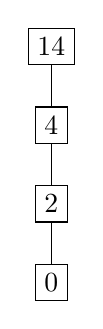
\begin{tikzpicture}
            \node[draw] (A) at (0,0) {14};
            \node[draw] (B) at (0,-1) {4};
            \node[draw] (C) at (0,-2) {2};
            \node[draw] (D) at (0,-3) {0};

            \draw (A) -- (B);
            \draw (C) -- (B);
            \draw (C) -- (D);

        \end{tikzpicture}
        \label{moncode}
    \end{center}
\end{frame}
\subsection{Optimalité}
\begin{frame}[fragile]
    \frametitle{Optimalité}

    \begin{center}
        \begin{lstlisting}[language=Python]
systeme = [30, 24, 12, 6, 3, 1]
\end{lstlisting}
        \captionof{code}{Système monétaire impérial britannique}
        \label{systeme}
    \end{center}
    \begin{activite}
        Dérouler à la main l'exécution de la fonction \textbf{\texttt{rendu\_monnaie}} pour 48€ avec le système impérial.
    \end{activite}
\end{frame}

\begin{frame}
    \frametitle{Correction}

    \begin{center}
        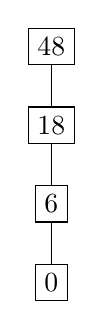
\begin{tikzpicture}
            \node[draw] (A) at (0,0) {48};
            \node[draw] (B) at (0,-1) {18};
            \node[draw] (C) at (0,-2) {6};
            \node[draw] (D) at (0,-3) {0};

            \draw (A) -- (B);
            \draw (C) -- (B);
            \draw (C) -- (D);
        \end{tikzpicture}
        \captionof{figure}{Solution donnée par l'algorithme glouton.}
    \end{center}

\end{frame}
\begin{frame}
    \frametitle{Une meilleure solution}

    \begin{center}
        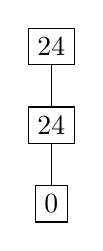
\begin{tikzpicture}
            \node[draw] (A) at (0,0) {24};
            \node[draw] (B) at (0,-1) {24};
            \node[draw] (C) at (0,-2) {0};

            \draw (A) -- (B);
            \draw (C) -- (B);
        \end{tikzpicture}
        \captionof{figure}{Une meilleure solution.}
    \end{center}

\end{frame}
\begin{frame}
    \frametitle{}

    \begin{aretenir}[Remarque]
    Le système monétaire européen garantit une solution optimale avec l'algorithme glouton. Ce système est dit \textbf{canonique}.
    \end{aretenir}

\end{frame}

\section{Approche dynamique}
\subsection{Algorithme naïf}
\begin{frame}
    \frametitle{Approche dynamique - Algorithme naïf}

    \begin{aretenir}[]
    Pour être certain de trouver la solution optimale, il faut calculer toutes les possibilités.\\Le principe d'optimalité de Bellman affirme qu'une solution optimale d'un problème s'obtient en combinant des solutions optimales à des sous-problèmes.
    \end{aretenir}

\end{frame}
\begin{frame}

    \begin{center}
        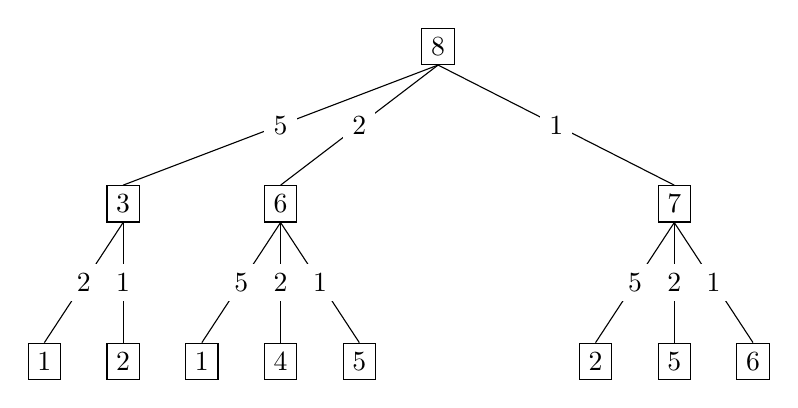
\begin{tikzpicture}
            \node[draw] (8-1) at(0,0){8};

            \node[draw] (3-2) at(-4,-2){3};
            \node[draw] (6-2) at(-2,-2){6};
            \node[draw] (7-2) at(3,-2){7};
            \draw (8-1.south) -- (3-2.north) node[midway, fill=white]{5};
            \draw (8-1.south) -- (6-2.north) node[midway, fill=white]{2};
            \draw (8-1.south) -- (7-2.north) node[midway, fill=white]{1};

            \node[draw] (1-4) at(-5,-4){1};
            \node[draw] (2-4) at(-4,-4){2};
            \draw (3-2.south) -- (1-4.north) node[midway, fill=white]{2};
            \draw (3-2.south) -- (2-4.north) node[midway, fill=white]{1};
            \node[draw] (1-42) at(-3,-4){1};
            \node[draw] (4-4) at(-2,-4){4};
            \node[draw] (5-4) at(-1,-4){5};
            \draw (6-2.south) -- (1-42.north) node[midway, fill=white]{5};
            \draw (6-2.south) -- (4-4.north) node[midway, fill=white]{2};
            \draw (6-2.south) -- (5-4.north) node[midway, fill=white]{1};

            \node[draw] (2-42) at(2,-4){2};
            \node[draw] (5-42) at(3,-4){5};
            \node[draw] (1-43) at(4,-4){6};
            \draw (7-2.south) -- (2-42.north) node[midway, fill=white]{5};
            \draw (7-2.south) -- (5-42.north) node[midway, fill=white]{2};
            \draw (7-2.south) -- (1-43.north) node[midway, fill=white]{1};
        \end{tikzpicture}
        \captionof{figure}{Rendre 8€}
    \end{center}

\end{frame}
\begin{frame}
    \frametitle{}

    \begin{center}
        \centering
        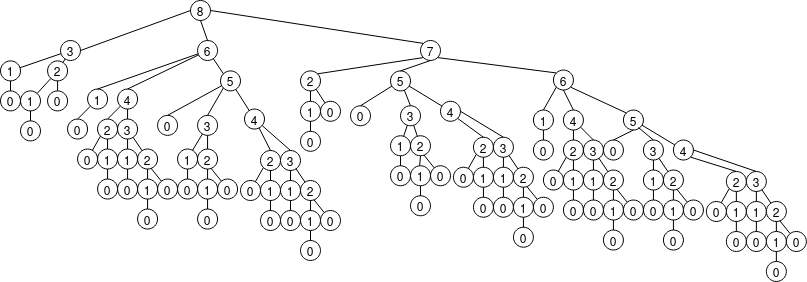
\includegraphics[width=10cm]{ressources/appel-naif-8.png}
        \captionof{figure}{Appels récursifs pour 8€}
        \label{IMG}
    \end{center}

\end{frame}
\begin{frame}[fragile]
    \frametitle{}

\begin{center}
\begin{lstlisting}[language=Python , basicstyle=\ttfamily\small, xleftmargin=0.2em, xrightmargin=-2em]
def rendu_naif(somme: int, systeme: list) -> list:
    if somme > 0:
        # somme = 1 + 1 + 1 ...
        mini = [1 for _ in range(somme)]  
        # Teste tous les possibles pour chaque pièce
        for piece in systeme:
            if piece <= somme:
                pieces = [piece] + \
                        rendu_naif(somme-piece, systeme)
                if len(pieces) < len(mini):
                    mini = pieces
        # garde le rendu minimum
        return mini
    else:
        return []
\end{lstlisting}
\end{center}
\end{frame}
\begin{frame}
    \frametitle{}

    
\begin{activite}
    \begin{enumerate}
        \item Dérouler le début de l'algorithme à la main pour en comprendre le fonctionnement.
        \item Ajouter une variable globale \textbf{\texttt{COMPTEUR}} qui compte le nombre d'appels récursifs.
    \end{enumerate}
    \end{activite}

\end{frame}
\begin{frame}[fragile]
\frametitle{Correction}
\begin{center}
\begin{lstlisting}[language=Python , basicstyle=\ttfamily\small, xleftmargin=0.2em, xrightmargin=-2em]
def rendu_naif(somme: int, systeme: list) -> list:
    global C
    if somme > 0:
        mini = [1 for _ in range(somme)] 
        for piece in systeme:
            if piece <= somme:
                C += 1
                pieces = [piece] + \
                        rendu_naif(somme-piece, systeme)
                if len(pieces) < len(mini):
                    mini = pieces
        # garde le rendu minimum
        return mini
    else:
        return []
\end{lstlisting}
\end{center}

\end{frame}
\begin{frame}[fragile]
    \frametitle{}

\begin{center}
\begin{lstlisting}[language=Python , basicstyle=\ttfamily\small, xleftmargin=0.2em, xrightmargin=2em]
>>> C = 0
>>> rendu_naif(14, [10, 5, 2, 1])
[10, 2, 2]
>>> C
2651
\end{lstlisting}
\end{center}

\end{frame}
\subsection{Approche descendante (top-down)}
\begin{frame}[fragile]
    \frametitle{Approche descendante (top-down)}

    \begin{activite}
    \begin{enumerate}
        \item Écrire la fonction \textbf{\texttt{rendu\_td(somme: int, systeme: list, track: list) $\rightarrow$ list}} qui s'inspire de la version naïve mais maintient un tableau \textbf{\texttt{track}} des solutions optimales pour chaque somme à rendre. Le tableau sera initialisé par:

        \begin{lstlisting}[language=Python , basicstyle=\ttfamily\small, xleftmargin=2em, xrightmargin=2em]
track = [[] for _ in range(somme+1)]
\end{lstlisting}
        \item Ajouter une variable globale \textbf{\texttt{COMPTEUR}} qui compte le nombre d'appels récursifs.
    \end{enumerate}
    \end{activite}

\end{frame}
\begin{frame}[fragile]

\begin{center}
\begin{lstlisting}[language=Python , basicstyle=\ttfamily\small, xleftmargin=0.2em, xrightmargin=-2.5em]
def rendu_td(somme: int, systeme: list, track: list) -> list:
    # le choix de pièces a déjà été calculé
    if len(track[somme]) > 0:
        return track[somme]
    elif somme > 0:
        mini = [1 for _ in range(somme)] 
        # Teste tous les possibles pour chaque pièce
        for piece in systeme:
            if piece <= somme:
                pieces = [piece] + \
                    rendu_td(somme-piece, systeme, track)
                if len(pieces) < len(mini):
                    mini = pieces
        # garde le rendu minimum
        track[somme] = mini
        return mini
    else:
        return []
\end{lstlisting}
\end{center}

\end{frame}
\begin{frame}[fragile]
    \frametitle{}

\begin{center}
\begin{lstlisting}[language=Python , basicstyle=\ttfamily\small, xleftmargin=2em, xrightmargin=2em]
>>> track = [[] for _ in range(s+1)]
>>> rendu_td(s, [10, 5, 2, 1], track)
[10, 2, 2]
\end{lstlisting}
\captionof{code}{Appel}
\label{CODE}
\end{center}

\end{frame}
\begin{frame}[fragile]
    \frametitle{}

\begin{center}
\begin{lstlisting}[language=Python , basicstyle=\ttfamily\small, xleftmargin=2em, xrightmargin=2em]
>>> C = 0
>>> track = [[] for _ in range(s+1)]
>>> rendu_td(s, [10, 5, 2, 1], track)
[10, 2, 2]
>>> C
42
\end{lstlisting}
\captionof{code}{Nombre d'appels récursifs}
\label{CODE}
\end{center}

\end{frame}
\begin{frame}
    \frametitle{}

    \begin{center}
    \centering
    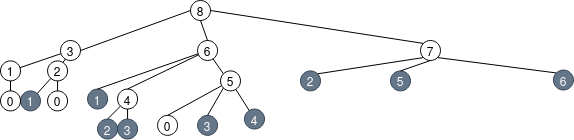
\includegraphics[width=10cm]{ressources/appel-dyn-8.png}
    \captionof{figure}{Approche dynamique pour 8€}
    \label{IMG}
    \end{center}

\end{frame}
\subsection{Approche ascendante (bottom-up)}
\begin{frame}[fragile]
    \frametitle{Approche ascendante (bottom-up)}

    \begin{activite}
        \begin{enumerate}
            \item Écrire la fonction \textbf{\texttt{rendu\_bu(somme: int, systeme: list) $\rightarrow$ list}} qui complète un tableau \textbf{\texttt{track}} des solutions optimales, en le remplissant d'abord par les plus petites sommes à rendre. Le tableau sera initialisé par:

\begin{lstlisting}[language=Python , basicstyle=\ttfamily\small, xleftmargin=2em, xrightmargin=2em]
track = [[] for _ in range(somme+1)]
\end{lstlisting}
            \item Ajouter une variable globale \textbf{\texttt{COMPTEUR}} qui compte le nombre d'appels récursifs.
        \end{enumerate}
    \end{activite}

\end{frame}
\begin{frame}[fragile]
    \frametitle{Correction}

\begin{center}
\begin{lstlisting}[language=Python , basicstyle=\ttfamily\small, xleftmargin=0.2em, xrightmargin=0em]
def rendu_bu(somme: int, systeme: list) -> list:
    track = [[] for _ in range(somme+1)]
    # pour chaque pièce de track on cherche le nombre minimum de pièces à rendre
    for x in range(1, somme+1):
        # on ne rend que des pièces de 1
        mini = [1 for _ in range(x)]
        for piece in systeme:
            if piece <= x:
                # prend la solution optimale pour 'x-piece'
                pieces = [piece] + track[x-piece]
                if len(pieces) < len(mini):
                    mini = pieces
        track[x] = mini

    return track[somme]
\end{lstlisting}
\end{center}  

\end{frame}
\begin{frame}[fragile]
    \frametitle{}

\begin{center}
\begin{lstlisting}[language=Python , basicstyle=\ttfamily\small, xleftmargin=2em, xrightmargin=2em]
>>> rendu_bu(s, [10, 5, 2, 1])
[10, 2, 2]
\end{lstlisting}
\captionof{code}{Appel}
\label{CODE}
\end{center}

\end{frame}
\begin{frame}[fragile]
    \frametitle{}

\begin{center}
\begin{lstlisting}[language=Python , basicstyle=\ttfamily\small, xleftmargin=0.2em, xrightmargin=0em]
track = [[], [1], [2], [2, 1], [2, 2], [5], [5, 1], [5, 2], [], [], [], [], [], [], []]
\end{lstlisting}
\captionof{code}{\centering État de \textbf{\texttt{track}} au début de l'itération \textbf{\texttt{x = 8}}}
\begin{lstlisting}[language=Python , basicstyle=\ttfamily\small, xleftmargin=0.2em, xrightmargin=0em]
for piece in systeme:
    if piece <= x:
        # prend la solution optimale pour 'x-piece'
        pieces = [piece] + track[x-piece]
        if len(pieces) < len(mini):
            mini = pieces
\end{lstlisting}
\captionof{code}{\centering Pour \textbf{\texttt{piece = 5}}, la variable \textbf{\texttt{pieces = [5] + [2, 1]}} }
\end{center}

\end{frame}
\begin{frame}[fragile]
    \frametitle{}

\begin{center}
\begin{lstlisting}[language=Python , basicstyle=\ttfamily\small, xleftmargin=2em, xrightmargin=2em]
>>> C = 0
>>> rendu_bu(s, [10, 5, 2, 1])
[10, 2, 2]
>>> C
42
\end{lstlisting}
\captionof{code}{Nombre d'appels récursifs}
\label{CODE}
\end{center}

\end{frame}
\end{document}